\chapter{Comparative Study}
\label{chap:comparative_study}

The version 1.2 of the TLS protocol was defined in RFC5246 in August 2008 und has been in use many years. With the release of TLS 1.3 in August 2018 some security and speed improvements of the protocol have been implemented. The TLS 1.3 is defined in RFC8446. In the following chapters the changes and differences of both TLS releases are examinated and discussed.

\section{Handshake/Speed improvement}
\label{sec:comparison_handshake}

\subsection{TLS 1.2 handshake}
\label{subsec:handshake1_2}

As described in the chapter ... (todo: add reference) the Handshake begins after the establishment of the TCP connection between client and server. The goals of the handshake protocol are to authenticate the server and, optionally, the client; negotiate protocol version, ciphersuites and extensions; derive authencticated encryption keys for the secure connection; ensure agreement on all negotiated parameters. \cite{Hassenstein}
The figure \ref{fig:handshake1_2} shows the process of the full handshake in the TLS protocol 1.2 for simplicity only with authentication of the server. There will be more steps of the handshake in case of the mutual authentication when the client must be also authenticated by the server.

\begin{figure}[H]
	\centering
		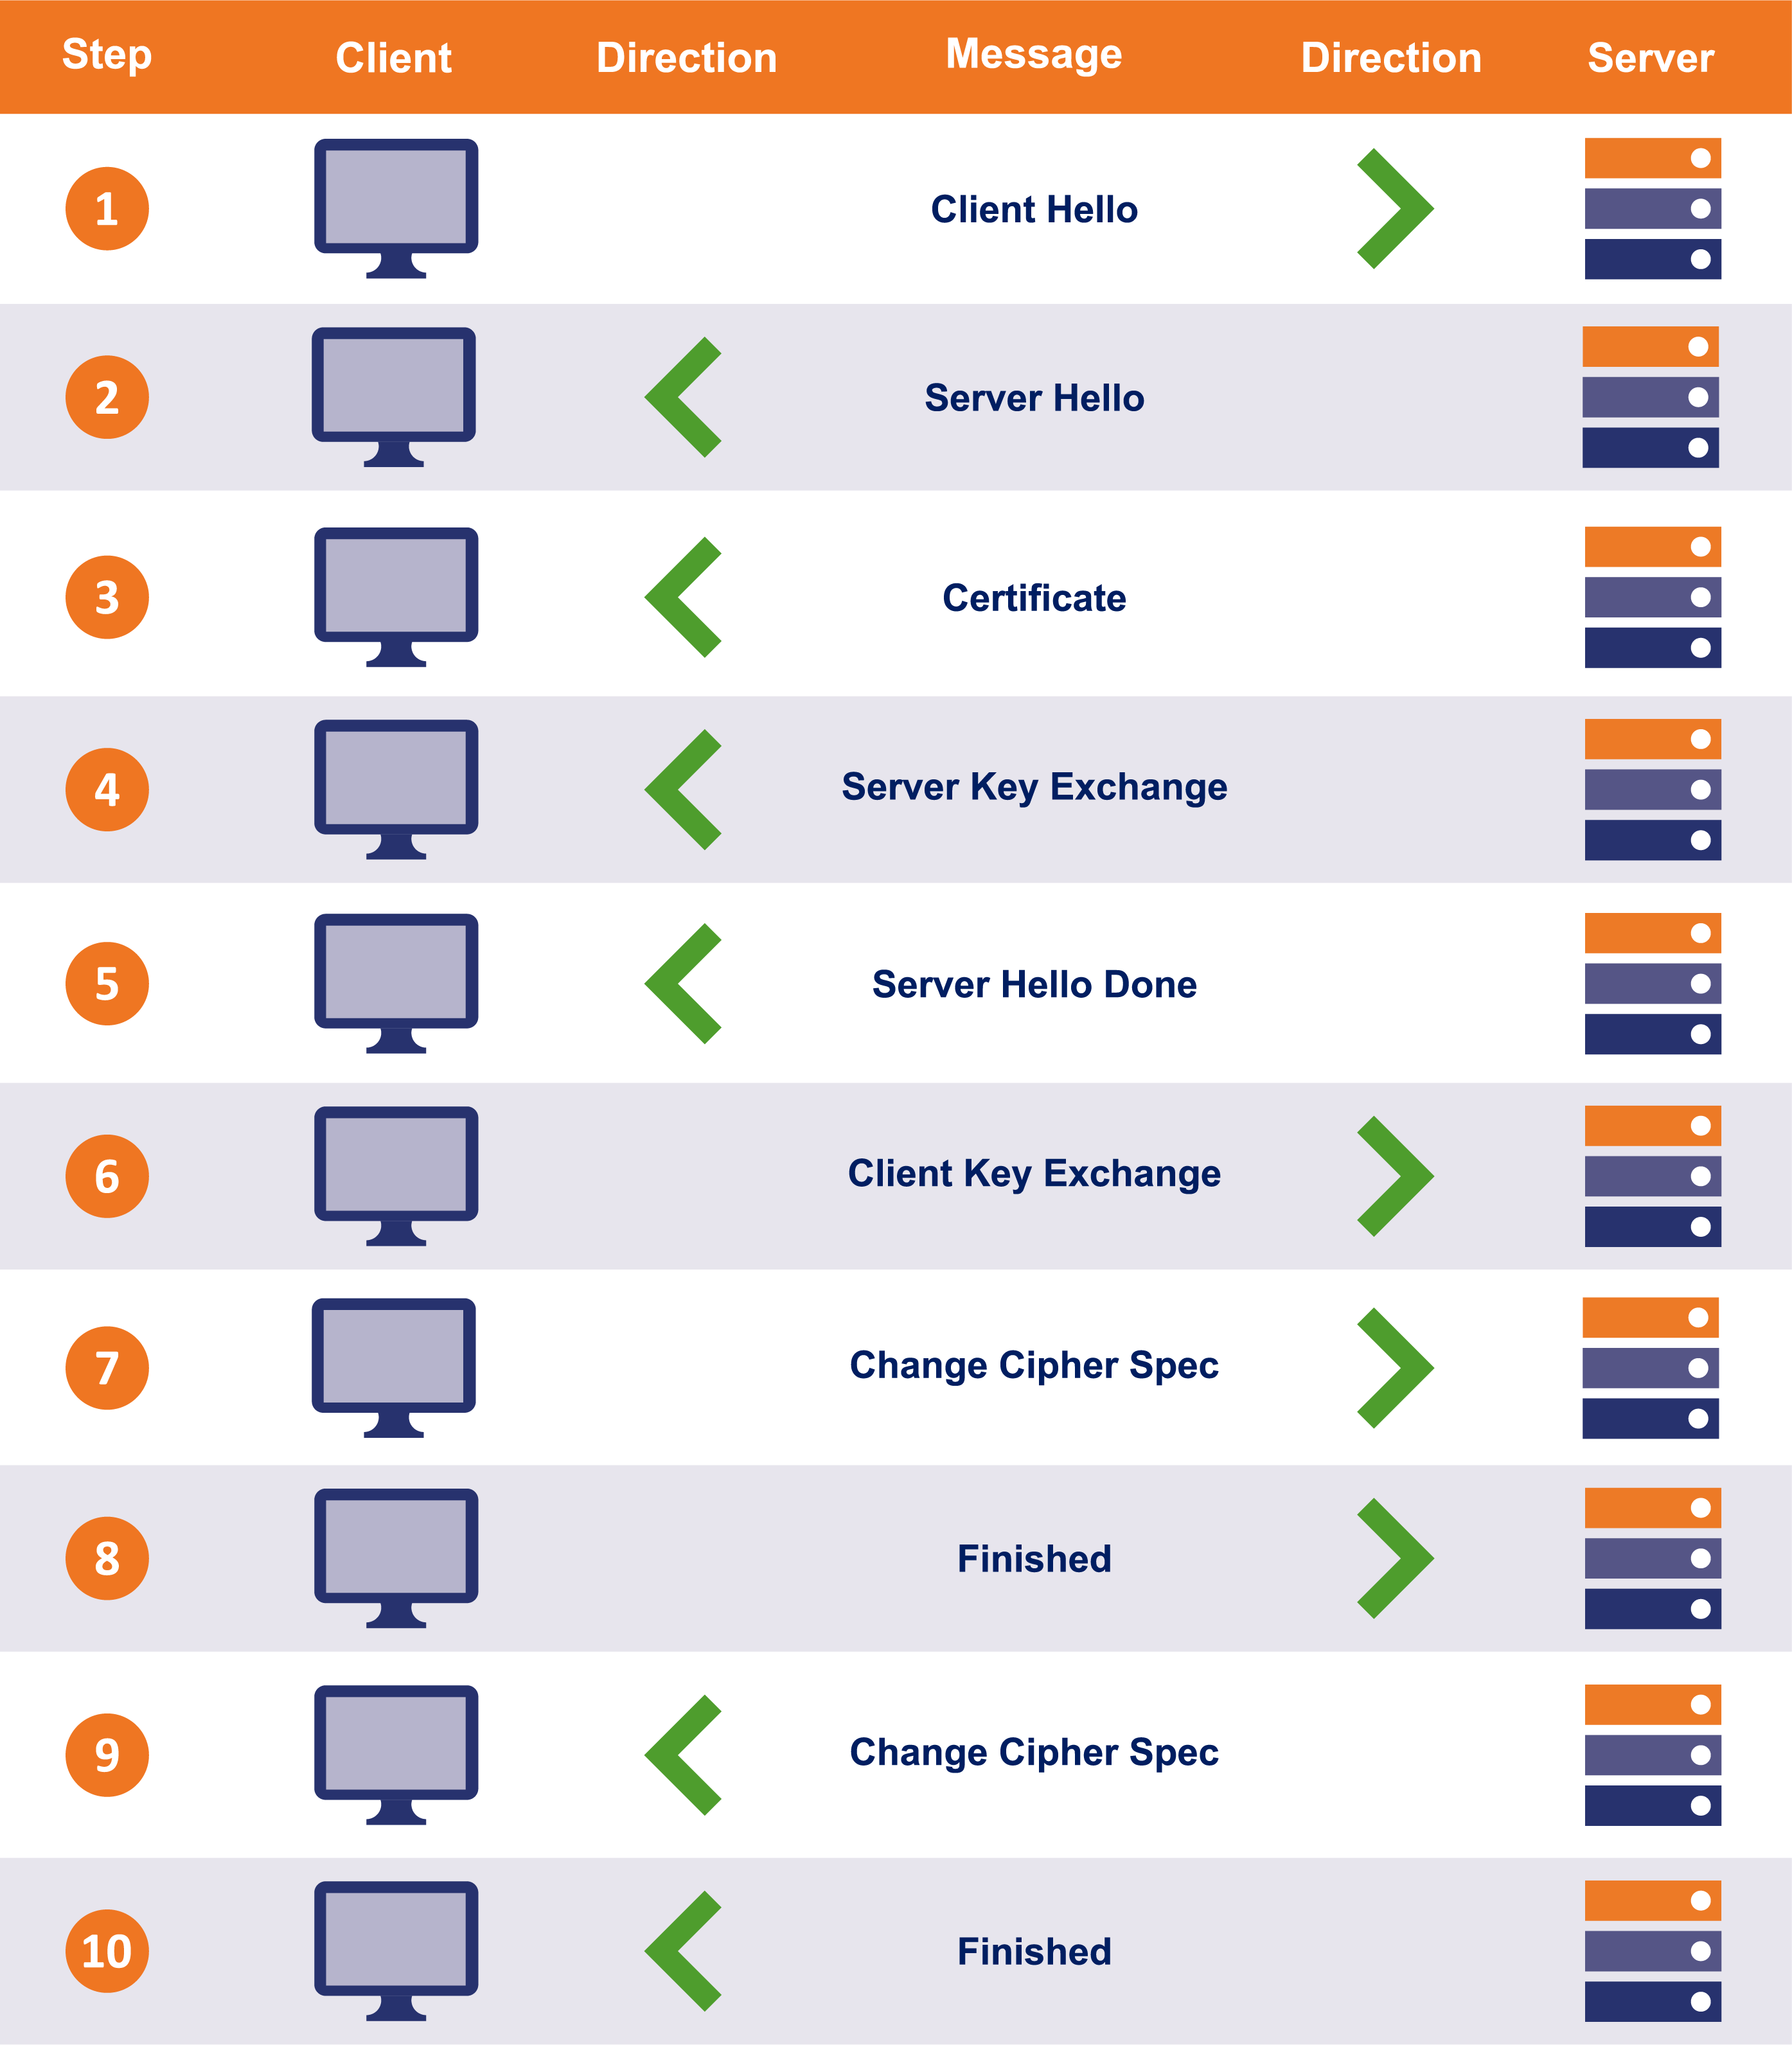
\includegraphics[scale=0.35]{images/handshake1_2.png}
	\caption{TLS 1.2 handshake with server authentication \cite{sslstore:handshake}}
	\label{fig:handshake1_2}
\end{figure}

\textbf{Step 1.} The 1th round of the handshake begins with the "client hello" message sent from the client to the server. This message includes the following cryptographic information:

\begin{itemize}
	\item CipherSuites - encryption algorithms supported by the client
	\item desired maximum of the protocol version
	\item random value generated on the client side
	\item session id
\end{itemize}

\textbf{Step 2.} Then the server responds with "server hello" message. The message consists of the following information:

\begin{itemize}
	\item CipherSuites chosen by the server from the "client hello" message
	\item protocol version supported by the server
	\item random value generated on the server side
	\item session id
\end{itemize}

\textbf{Step 3.} The server sends its X.509 certificate and its public key.

\textbf{Step 4.} This step is needed if the Diffie-Hellmann key exchange algorithm was negotiated between the client and the server at the steps 1 and 2. In this case the server transmits additional key materials in the "server key exchange" message.

\textbf{Step 5.} With the "server hello done" message the server notify the client that it finished his steps and wait on the answer of the client.

\textbf{Step 6.} The client verifies the certificate sent by the server. Then it transmit to the server its key material in the key exchange message. 
At this point the client and the server can compute pre-master secret from key exchange messages. Using the pre-master secret with the nonces sent in the steps 1 and 2 they can generate the master key. Afterwards the client and the server derive a set of session keys from the master key that will be used to symmetrically encrypt the data.

\textbf{Step 7.} Wenn the client derived the session key it notify the server about the change of the keys for the secure communication.

\textbf{Step 8.} With the message "Finished" the client signals to the server that it completed its tasks and is ready for the communication. This message includes MAC of the messages from the previous steps using the calculated master key, so that the server can verify integrity of the handshake's messages.

\textbf{Step 9-10.} The server makes the same steps as the client in the steps 7-8 to switch the keys for the symmetric encryption and notifies the client with the message "finished". This message includes the MAC of the whole handshake log except "change cipher spec" messages from the steps 7 and 9. \cite{sslstore:handshake}\cite{Hassenstein}

The almost whole communication in the handshake protocol flows in the clear text. Only beginning from the step 8, when the client finished his preparation for the secure communication, the next messages of the handshake will be encrypted.

\subsection{TLS 1.3 handshake}
\label{subsec:handshake1_3}

\begin{figure}[H]
	\centering
		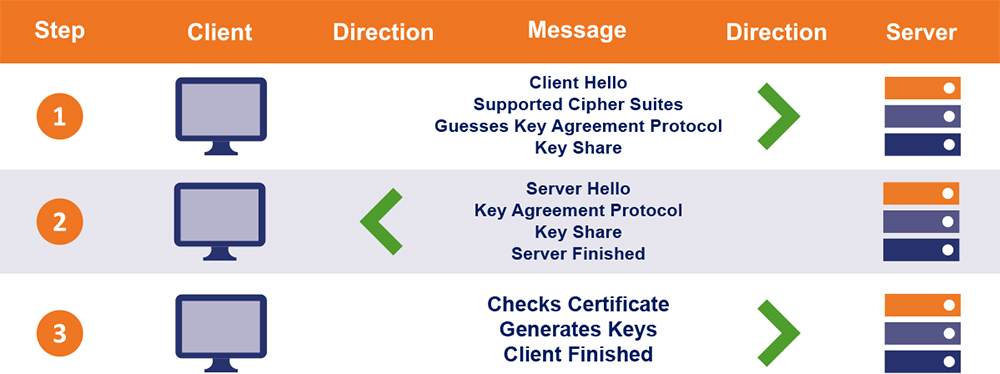
\includegraphics[scale=0.35]{images/handshake1_3.jpg}
	\caption{TLS 1.3 handshake \cite{sslstore:handshake}}
	\label{fig:handshake1_3}
\end{figure}

\textbf{Step 1.} The TLS 1.3 handshake begins with the "client hello" message as in the TLS 1.2 handshake. In addition the client sends in the same message the following information:

\begin{itemize}
	\item the list of the supported CypherSuites
	\item key share entries consisting of a named (EC)DH group and an ephemeral public key
\end{itemize}

\textbf{Step 2.} The server respondes with the "server hello" message. In addition it sends the following information:

\begin{itemize}
	\item chosen CypherSuite
	\item key share entries consisting of the chosen (EC)DH group and its public key
	\item the certificate of the server
	\item "certificate verify" message containing a hash of all previous handshake messages signed with the private key of the server. The client afterwards verifies the signature with the public key from the server's certificate. 
	\item "server finished" message
\end{itemize}

In case if the server does not support any of the proposed groups the server will request retrying the handshake or abort the connection with a fatal handshake\_failure alert.

\textbf{Step 3.} The client checks the certificate of the server. Generates keys from the key share of the server from the previous step. Afterwards the client sends the "client finished" message. \cite{Hassenstein}\cite{sslstore:handshake}

After the "server hello" message all handshake messages will be encrypted.

\subsection{Discussion of TLS 1.2 and 1.3 full handshakes (todo: change title)}
\label{subsec:comparison_handshake}

The TLS 1.2 handshake takes two round trips between the client and the server to complete the handshake. On average, this process requires 0.25 to 0.5 seconds.

The "server key exchange" and "client key exchange" messages have been removed from the TLS 1.3 handshake. The key exchange parameters and public keys will be sent in the key share extensions, that are added to the "client hello" and "server hello" messages. This keeps the 1.3 release compatible with the 1.2 version because the order of messages remains.

Furthermore the ChangeCipherSpec protocol has been removed in the 1.3 version. 

As a consequence of this the TLS 1.3 handshake involves only one round trip. This changes results in reduced latency almost in half. As mentioned in the blog of The SSL Store a delay of half a second results in 20\% traffic decline \cite{sslstore:handshake}. That is why the performance improvement of the TLS protocol is a crucial change in the protocol.

Moreover the privace of the handshake protocol has been improved. In the 1.2 release of the TLS protocol almost all handshake messages are sent in the clear text except the last steps after the client sends "finished" message. On the contrary in the 1.3 version all information will be encrypted as early as possible, namely after "server hello" message. 

\section{Session resumption}
\label{sec:resumption}

The full handshake can take time, increase server load and cause connection latency. To improve performance the session resumption can be used. With the "client hello" and "server hello" messages the session id can be saved and used to resume previously established TLS session. Under this session id the client and the server store the master key and other details of the connection. In the next session they can transmit the session id and thus reuse past connection parameters. The following session data can be cached: master secret, protocol version, ciphersuits, compression method, certificate.





\section{Overview}
\label{sec:overview}

\begin{table}[H]
	\centering
		\begin{tabular}{lll} \toprule
			\textbf{Characteristic} & \textbf{TLS 1.2} & \textbf{TLS 1.3} \\ \midrule
			Round trip time of the full handshake & 2-RTT & 1-RTT \\ \midrule
			Encryption of handshake messages& at the end, & at the beginning, \\ 
			& after "client finished" message & after "server hello" message \\ \midrule
			Speed of the full handshake & 0.25-0.5 s & 0.2-0.3 s\\ \midrule
		\end{tabular}
	\caption{Comparison of TLS 1.2 and TLS 1.3}
	\label{tab:comparison}
\end{table}

